% !TEX root = ../main.tex
%
\chapter{Background}
\label{sec:background}

\section{View Synthesis}

View synthesis is a fundamental technique in applications ranging from virtual reality to digital filmmaking.
It involves generating new views of a scene from images captured at different viewpoints, aiming to produce photorealistic outputs that were not originally captured by cameras.

\paragraph{Mesh-based Methods}

View synthesis methods based on mesh representations typically construct a geometric mesh to model the scene \cite{levoy_light_1996,gortler_lumigraph_1996,zitnick_high-quality_2004,debevec_modeling_1996,buehler_unstructured_2001,chen_view_1993}.
This mesh is then used as a framework upon which textures from various captured viewpoints are mapped.
The success of this approach heavily relies on the precision of the mesh construction and the accuracy of the texture alignment.
These methods are particularly effective in controlled environments where detailed and accurate geometric data can be assured, making them ideal for high-quality visual effects in movies and games.

\paragraph{Volumetric Methods}

In contrast to mesh-based methods, volumetric view synthesis techniques represent the scene using a spatial grid that encapsulates the volume of the space.
\cite{seitz_photorealistic_1999,curless_volumetric_1996}
These methods are less dependent on precise geometry and are capable of handling complex topologies and incomplete data sets.
They work by interpolating the volumetric space to synthesize new views, which makes them well-suited for dynamic environments where rapid processing of unstructured data is required.

\section{Neural Approaches to View Synthesis}

Neural networks provide a powerful framework for view synthesis, representing a significant advancement over traditional methods which involve multiple complex stages of processing. 
These networks are particularly adept at learning the mappings required to synthesize new views directly from images.

\paragraph{Direct Pixel Prediction}
Traditional neural approaches involve models that predict pixel values directly from input images. 
These methods simplify the synthesis pipeline by eliminating intermediate stages, thus reducing potential errors and computational overhead \cite{flynn_deep_2016}.

\paragraph{Depth and Geometry Estimation}
Some neural methods estimate depth or 3D structures from images, using this geometric information to aid in generating new views. 
This step often involves convolutional neural networks and emphasizes the geometry reconstruction aspect of view synthesis \cite{eigen2014depth}.

\paragraph{Adversarial and Generative Models}
Generative adversarial networks (GANs) and other generative models have also been used to enhance the realism of synthesized views. 
These models learn to generate new images that are indistinguishable from real images, improving the photorealism of synthesized views \cite{goodfellow2014generative}.


Despite their advantages, neural models, including those used for view synthesis, require substantial computational power and data for training. This can be a barrier to their practical deployment, especially in resource-constrained environments \cite{canziani2016analysis}.
The performance of models like NeRF heavily depends on the availability of high-quality training data. Insufficient or biased data can severely limit the model's ability to generalize to new environments or scenarios \cite{torralba2011unbiased}.

Future research in neural view synthesis is likely to focus on improving the computational efficiency of models and reducing their reliance on extensive training datasets. Techniques such as network pruning and transfer learning are being explored to address these issues \cite{han2015deep}.
Extending neural view synthesis methods to more complex scenarios, such as dynamic scenes and interactive media, is another critical area of research. This involves adapting models to handle temporal variations and interactive user inputs \cite{kopf2014first}.

\section{Neural Radiance Fields (NeRF)}

NeRF represents a significant advancement in neural view synthesis by modeling complex scenes as continuous volumetric fields. Introduced by Mildenhall et al., NeRF utilizes a deep fully connected network, or multilayer perceptron (MLP), to map 5D coordinates—consisting of spatial locations and viewing directions—to the volume density and radiance at those points \cite{mildenhall2020nerf}.

\subsection*{Technical Implementation}
\paragraph{Scene Representation}
NeRF models a scene using a continuous 5D function where each input, a combination of 3D spatial coordinates and 2D viewing directions, is associated with an output comprising volume density and view-dependent emitted radiance. This approach enables the rendering of intricate details by effectively capturing the light interaction within the scene.

\paragraph{Differentiable Volume Rendering}
The core of NeRF's rendering technique lies in differentiable volume rendering. For each viewpoint, rays are traced through the scene, sampling points along each ray. These points, represented as 5D coordinates, are input into the MLP, which outputs the color and density for each point. The rendered image is then produced by compositing these outputs using classical volume rendering formulas, which are naturally differentiable and thus suitable for gradient-based optimization.

\paragraph{Positional Encoding}
To enhance the MLP's ability to model high-frequency functions and represent finer details, the input coordinates are transformed through a positional encoding before being fed into the network. This encoding increases the model's capacity to differentiate between minute variations in input data, crucial for accurately rendering complex geometries and textures.

\subsection{Optimization Process}
NeRF is optimized by minimizing the photometric error between the rendered images and the corresponding ground-truth images across multiple views. This optimization encourages consistency and coherence in the rendered views, ensuring that the neural radiance fields accurately represent the underlying scene content.

\paragraph{Hierarchical Sampling}
To efficiently handle the vast amount of data and improve the convergence rate, NeRF employs a hierarchical sampling strategy. This involves using two networks—a coarse and a fine network—to progressively refine the predictions of density and color at sampled points along the rays.

\subsection*{Advantages Over Previous Methods}
Compared to prior methods, NeRF can generate photorealistic images from a sparse set of input views while being highly memory efficient. Unlike discrete voxel grid approaches, which suffer from high memory usage and poor scaling with resolution, NeRF’s continuous representation allows for more detailed and higher resolution outputs.

\subsection*{Challenges and Limitations}
While NeRF provides impressive results, it is computationally intensive, requiring significant resources for training and inference. Furthermore, NeRF assumes a static scene and thus struggles with dynamic objects or lighting changes.

\subsection*{Future Directions}
The adaptability of NeRF to more general applications, including dynamic scenes and interactive settings, is an active area of research. Enhancements to reduce computational demands and improve real-time performance are also critical for broader adoption.


% \section{Neural Radiance Fields (NeRF)}

% Neural Radiance Fields (NeRF) have emerged as a transformative approach to view synthesis, enabling the rendering of complex scenes with unprecedented realism. 
% Introduced by \cite{mildenhall_nerf_2021}, NeRF utilizes a deep neural network to model a continuous volumetric scene function that is optimized directly from a set of sparse input views. 
% This method represents a significant advancement over traditional techniques of neural 3D shape representation 

% The core innovation of NeRF lies in its ability to handle complex geometries and material properties by encoding the scene in a high-dimensional space defined by spatial location and viewing direction. 
% Positional encoding of the input coordinates allows the model to capture high-frequency details, crucial for rendering realistic images \cite{mildenhall_nerf_2021}. 
% Additionally, NeRF's use of volume rendering techniques facilitates the projection of computed radiance and density into images, enabling it to overcome the storage limitations associated with voxel grids.

% \begin{figure}[htb]
%   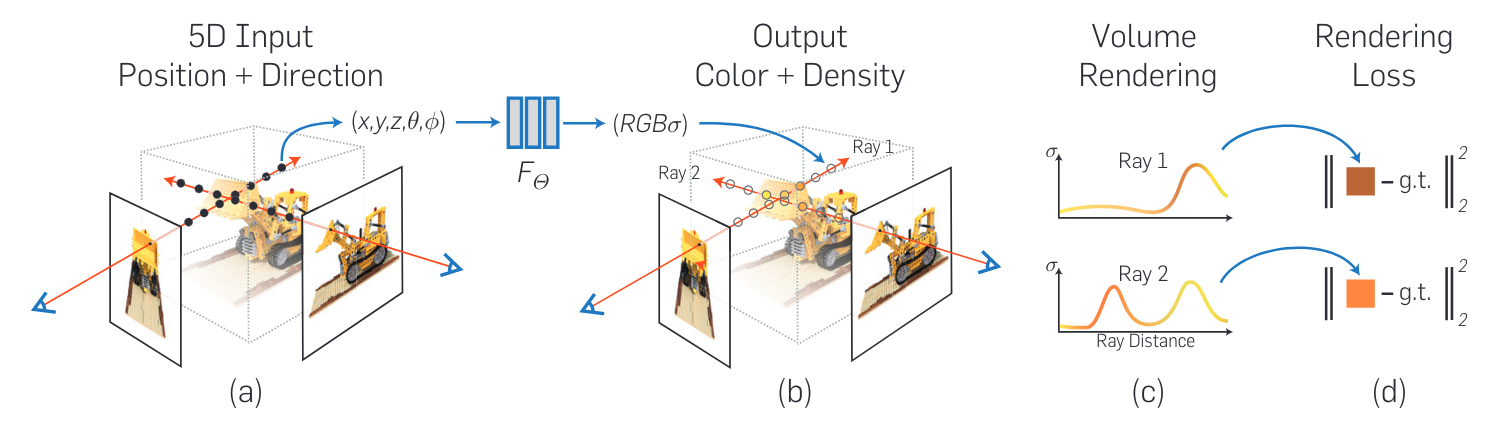
\includegraphics[width=\textwidth]{figures/bg-nerf.png}
%   \caption{NeRF Scene Representation}
%   \label{fig:background:nerf}
% \end{figure}


% Despite its advantages, NeRF's application to real-world scenarios is not without challenges. 
% The lengthy optimization times, the static nature of scenes, and the handling of highly dynamic environments are areas ripe for further research. 
% Future work could explore more efficient training methods, extensions to dynamic scenes, and the integration of NeRF with other cutting-edge AI technologies to enhance its functionality and applicability in practical applications.

% % \subsection{Applications in the Film Industry}
% NeRF's ability to synthesize photorealistic scenes from sparse datasets can significantly benefit the film industry by reducing the reliance on physical sets and manual post-processing, thereby optimizing costs and production times. % Add references to case studies or reports on NeRF's applications in film

% \section{Conclusion}
% This chapter discussed the transformative role of NeRF in view synthesis, particularly its potential to revolutionize scene creation in the film industry. The integration of such advanced technologies promises to enhance not only the visual quality but also the efficiency of film production workflows.
